\documentclass[conference]{IEEEtran}
\IEEEoverridecommandlockouts
% The preceding line is only needed to identify funding in the first footnote. If that is unneeded, please comment it out.
\usepackage{cite}
\usepackage{amsmath,amssymb,amsfonts}
\usepackage{algorithmic}
\usepackage{graphicx}
\usepackage{textcomp}
\usepackage[x11names]{xcolor}
\usepackage{gensymb}
\usepackage{wasysym}
\usepackage{graphics}
\usepackage{bm}
\usepackage{xfrac}
\usepackage{siunitx}
\usepackage{pgfplots}
\usepackage{tikz, tikz-3dplot}
\usepackage{xfp}
\usepackage{dutchcal}
\usepackage{float}
\usepackage{hyperref}
\hypersetup{
	colorlinks=true,
	linkcolor=black,
	filecolor=magenta,      
	urlcolor=SlateGray4,
	}
\def\BibTeX{{\rm B\kern-.05em{\sc i\kern-.025em b}\kern-.08em
	T\kern-.1667em\lower.7ex\hbox{E}\kern-.125emX}}
\graphicspath{ {./} }
\makeatletter
\newcommand*{\overrightharpoonup}{\mathpalette{\overarrow@\rightharpoonupfill@}}
\newcommand*{\rightharpoonupfill@}{\arrowfill@\relbar\relbar\rightharpoonup}
\makeatother
\renewcommand{\vec}[1]{\overrightharpoonup{\bm{\mathrm{#1}}}}
\newcommand{\vhat}[1]{\hat{\bm{\mathrm{#1}}}}
\newcommand{\abs}[1]{\lvert#1\rvert}
\newcommand{\norm}[1]{\abs{\abs{\vec{#1}}}}

\begin{document}

	\sisetup{per-mode = fraction, fraction-function = \sfrac}
	\sisetup{exponent-product = \ensuremath { { } \cdot { } } }

	\title{Two-Line Element Decoder and Visualizer\\
		{\footnotesize UNM ECE 535 Final Project: Software Type}
	}

	\author{\IEEEauthorblockN{Sonny Ji}
		\IEEEauthorblockA{\textit{Department of Electrical and Computer Engineering} \\
		\textit{The University of New Mexico}\\
		Albuquerque, United States \\
		velten@unm.edu}
	}

	\maketitle

	\begin{abstract}
		This document details the conceptualization, design, implementation, and finalization of a software tool for visualizing the orbits of satellites. The goal of this tool is to aid in the visualization of satellites and their orbits, along with a presentation that promotes a human-digestible format for better intuition and understanding of satellite orbital mechanics and satellite communication ranges.
	\end{abstract}

	\begin{IEEEkeywords}
		satellite communications, TLE, orbital mechanics, 3D-simulation, software
	\end{IEEEkeywords}

	\section{Introduction}
		This is a project for the ECE 535 Satellite Communications class at The University of New Mexico's Department of Electrical and Computer Engineering. The goal of this project is to develop and build a desktop application for decoding two-line element sets and representing the results in an interactive 3D graphic that tracks the satellite. Additionally, this tool will attempt to further append satellite information through pinging web-based APIs for further satellite information and data. This would include items (when applicable) such as: orbit lines, satellite use and type, cone of coverage, trajectory, Earth for scale, and visualizations of all 6 classical orbital mechanics parameters. The deliverable for this project is an application / software package for taking in two-line element sets as an input and presenting 3D models of the previously described as an output, along with a brief guide on how to use and interpret the tool.

		Information on the tool and a guide on how to use it are included at the end of this document under the \textit{Usage Information and Notes} section.

	\section{Useful Information and Definitions}

		\subsection{Abbreviations and Acronyms}\label{AA}
			\begin{itemize}
				\item TLE: Two-Line Element
				\item AN: Ascending Node
				\item DN: Descending Node
				\item RAAN: Right Ascension of the Ascending Node
			\end{itemize}

		\subsection{Variables and Symbols}
			\begin{itemize}
				\item \( a \): Semi-major axis of elliptical orbit
				\item \( b \): Semi-minor axis of elliptical orbit
				\item \( e \): Eccentricity of elliptical orbit
				\item \( i \): Inclination of elliptical orbit
				\item \( \Omega \): RAAN, longitude of the ascending node
				\item \( \omega \): Argument of periapsis of elliptical orbit
				\item \( \nu \): True anomaly of elliptical orbit
				\item \( \aries \): First point of Aries, vernal equinox
				\item \( \ascnode \): AN
				\item \( \descnode \): DN
				\item \( M \): Mean anomaly of elliptical orbit
				\item \( E \): Elliptical anomaly of elliptical orbit
				\item \( n_0 \): Mean motion of elliptical orbit
				\item \( R \): Radius of celestial body
				\item \( r \): Radius of orbit with respect to central orbiting body
			\end{itemize}

		\subsection{Subscripts}
			\begin{itemize}
				\item \( \cdot_a \): Relating to the apoapsis of an orbit
				\item \( \cdot_p \): Relating to the periapsis of an orbit
				\item \( \cdot_{\oplus} \): Relating to the Earth
				\item \( \cdot_0 \): Relating to epoch
			\end{itemize}

		\subsection{Units}
			\begin{itemize}
				\item All distances (i.e. \( a \), \( r_p \), \( R_{\oplus} \), etc.) are presented in kilometers
				\item All velocities (i.e. \( v_p \), \( v_a \), \( \vec{v} \), etc.) are presented in kilometers per second
				\item All angles (i.e. \( \nu_0 \), \( E_0 \), \( M_0 \), etc.) are presented in radians
				\item All angular velocities (i.e. \( \omega_{\oplus} \), \( n \), etc.) are presented in radians per second
				\item All durations (i.e. \( \Delta t \), etc.) are presented in seconds
			\end{itemize}

		\subsection{Constants}
			\begin{itemize}
				\item \( R_{\oplus}=\qty{6378}{\kilo\meter} \)
				\item \( \omega_{\oplus}=\qty{7.2921159e-5}{\radian\per\second} \)
				\item \( \mu_{\oplus}=\qty{3.986e5}{{\kilo\meter^3}\per{\second^2}} \)
			\end{itemize}

	\section{Motivations and Methodologies}

		\subsection{Motivations}
			As someone with a background in mechanical engineering, I found the orbital mechanics section of ECE 535 incredibly interesting. However, I wanted something to help me, and others with the same problems, visualize satellites and their orbits. Since the position of a satellite in a 3D orbit is somewhat difficult to grasp if it's your first exposure to the concept, a tool that helps bridge the gap between just understanding the math and numerical values behind the satellite, and gaining an intuition for how those numbers would actually affect a satellite and its orbit without having to do multiple orbital mechanics calculations, would be incredibly useful for students and anyone else just starting out in orbital mechanics. So, for my project, I decided to create a tool to visualize satellites and their orbits.
			
			Additionally, this program also helps to provide a tool to decode and interpret TLEs. Since TLEs contain all of the important information relevant to positioning a satellite in an orbit around the Earth, they serve as a great tool for user data input for selecting a satellite to visualize. Thus, I also decided to include a TLE ``translator'' in this project as well. Overall, the reason this project is important is that it will be a very useful tool for students learning about orbits and satellite communications to help give a more graphical and intuitive understanding of how satellites are positioned where they are, and how that affects the world.

		\subsection{Methodologies}
			While there are many orbit visualizers and simulators out there, a game called Kerbal Space Program was incredibly helpful for me in understanding orbits and satellites through its representation of orbits in a 3D interactive model, and definitely helped me gain a somewhat-intuitive understanding of orbital mechanics and the philosophies and principles behind the design, construction, and maintenance of communication satellites and satellite networks. Thus, I decided to expand on Kerbal Space Program and make my own visualization method specifically for ECE 535 roughly based on Kerbal Space Program's graphical representations.

			Furthermore, I decided to use Unity as the central graphics engine for this project. This is because Unity is a widely-used 3D game development platform and rendering engine, with a very wide compatibility for what machines it could compile and build for. Additionally, due to its large amount of user-generated help and support forums, along with its documentation for how to use and program for the Unity ecosystem, it seemed like a good way to both learn the fundamentals of Unity while also producing a helpful tool for the final project of ECE 535.

	\section{Implementation Philosophy and Ontology}
		The high-level goal of this project is to create a tool that visualizes the six classical orbital elements: \( a \), \( e \), \( i \), \( \Omega \), \( \omega \), and \( \nu \). The tool must also represent these quantities graphically, in a way that demonstrates exactly what the variable is measuring. Additionally, the tool must visualize celestial elements that help a student's understanding and intuition: \( \aries \), \( \ascnode \), \( \descnode \). Finally, the tool must take a full, correctly formatted TLE as an input.

	\section{Governing Physics and Equations}

		\subsection{Background for General Orbital Mechanics}
			A satellite's orbit around the Earth can be fully described through the six orbital elements. 

			The first orbital element, \( a \), is the semi-major axis of the orbit. This is useful in determining approximately how large an orbit is. Additionally, it is also the semi-major axis of the ellipse as seen from directly above the orbital plane, or in the negative \( \vhat{W} \) direction in the perifocal coordinate system, as demonstrated in Fig.~\ref{figA}.

			\begin{figure}[hbtp]
				\begin{center}
					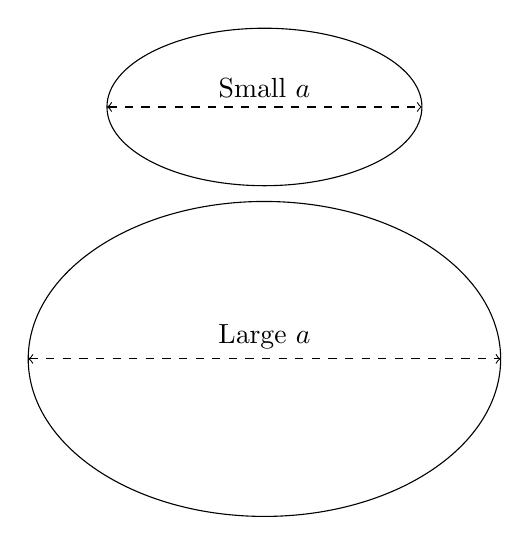
\begin{tikzpicture}[scale=1]
						\pgfmathsetmacro{\o}{1.6}
						\draw (0,\o) ellipse (2 and 1);
						\draw [<->, dashed] (-2,\o) -- (2,\o);
						\node at (0,\o) [anchor=south] {Small \( a \)};

						\draw (0,-\o) ellipse (3 and 2);
						\draw [<->, dashed] (-3,-\o) -- (3,-\o);
						\node at (0,-\o) [anchor=south] {Large \( a \)};
					\end{tikzpicture}
				\end{center}
				\caption{Small and large semi-major axes.}
				\label{figA}
			\end{figure}

			The second orbital element, \( e \), is the eccentricity of the orbit. This is useful in determining the aspect ratio of the orbit, or how ``squished'' an elliptical orbit is. Additionally, it is also the eccentricity of the ellipse created by the orbit as demonstrated in Fig.~\ref{figB}.

			\begin{figure}[hbtp]
				\begin{center}
					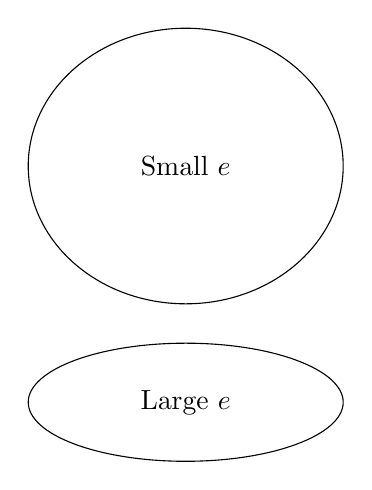
\begin{tikzpicture}[scale=1]
						\pgfmathsetmacro{\o}{1.5}
						\draw (0,\o) ellipse (2 and 1.75);
						\node at (0,\o) [anchor=center] {Small \( e \)};

						\draw (0,-\o) ellipse (2 and 0.75);
						\node at (0,-\o) [anchor=center] {Large \( e \)};
					\end{tikzpicture}
				\end{center}
				\caption{Small and large eccentricities.}
				\label{figB}
			\end{figure}

			The third orbital element, \( i \), is the inclination of the orbit. This is useful in determining the tilt of the orbit from the celestial equatorial plane as demonstrated in Fig.~\ref{figC}.

			\begin{figure}[hbtp]
				\begin{center}
					\tdplotsetmaincoords{80}{180}
					\begin{tikzpicture}[tdplot_main_coords, scale=2]
						\pgfmathsetmacro{\o}{1.5}
						\coordinate (O) at (0,0,0);
						\tdplotsetrotatedcoords{0}{15}{0}
						\tdplotdrawarc[color=black, fill=black, opacity=0.1, dashed]{(O)}{1}{0}{360}{anchor=north west, opacity=0.5}{Celestial Equator}
						\tdplotdrawarc[tdplot_rotated_coords, color=red, fill=red, opacity=0.1]{(O)}{1}{0}{360}{anchor=south west, opacity=0.5}{Orbital Plane}
						\tdplotsetrotatedcoords{90}{90}{90}
						\tdplotdrawarc[tdplot_rotated_coords, color=blue, ->]{(O)}{1}{0}{15}{anchor=west}{Small \( i \)}
					\end{tikzpicture}

					\tdplotsetmaincoords{80}{180}
					\begin{tikzpicture}[tdplot_main_coords, scale=2]
						\pgfmathsetmacro{\o}{1.5}
						\coordinate (O) at (0,0,0);
						\tdplotsetrotatedcoords{0}{50}{0}
						\tdplotdrawarc[color=black, fill=black, opacity=0.1, dashed]{(O)}{1}{0}{360}{anchor=north west, opacity=0.5}{Celestial Equator}
						\tdplotdrawarc[tdplot_rotated_coords, color=red, fill=red, opacity=0.1]{(O)}{1}{0}{360}{anchor=south west, opacity=0.5}{Orbital Plane}
						\tdplotsetrotatedcoords{90}{90}{90}
						\tdplotdrawarc[tdplot_rotated_coords, color=blue, ->]{(O)}{1}{0}{50}{anchor=west}{Large \( i \)}
					\end{tikzpicture}
				\end{center}
				\caption{Small and large inclinations.}
				\label{figC}
			\end{figure}

			The fourth orbital element, \( \Omega \), is the RAAN, or the longitude of the AN\@. It is the angle between \( \aries \) and \( \ascnode \) measured as a positive rotation on the celestial equator, or eastward from \( \aries \). This is useful in determining how rotated an orbit is on Earth's equator as demonstrated in Fig.~\ref{figD}. Because the stars and constellations generally don't move appreciably on a human timescale, the standard coordinate system used is based on the position of the stars and is called the celestial coordinate system. The first two planes of importance for celestial mechanics are the celestial equatorial plane, or the plane created by the Earth's equator, and the ecliptic plane, or the plane created by the Earth's orbit around the Sun. For Earth-orbiting satellites, the celestial equatorial plane is always used as the reference plane that the orbital elements are measured off of. Additionally, this system has a reference direction, designated \( \vhat{I} \), in the direction of the vernal equinox or the First Point of Aries, \( \aries \). This direction is determined when the line created by the intersection of the celestial equatorial plane and the ecliptic plane perfectly points toward the gravitational center of the Sun, meaning the Sun is coplanar with both the equatorial plane and the ecliptic plane. Specifically, the \( \aries \) vector points towards the Sun when the Sun appears to move from the Southern Hemisphere towards the Northern Hemisphere. Finally, the last plane of interest for orbital mechanics is the orbital plane, or the plane created by a satellite's orbit around the Earth. The intersection of the orbital plane and the equatorial plane creates a line called the line of nodes. The points at which this line intersects the satellite's orbit are labeled the AN, or \( \ascnode \), and DN, or \( \descnode \). Specifically, the AN is the point when the satellite crosses from below the equatorial plane to above it, and the DN is the point when the satellite crosses from above the equatorial plane to below it.

			\begin{figure}[hbtp]
				\begin{center}
					\tdplotsetmaincoords{65}{30}
					\begin{tikzpicture}[tdplot_main_coords, scale=2]
						\pgfmathsetmacro{\o}{45}
						\coordinate (O) at (0,0,0);
						\tdplotsetrotatedcoords{-\o}{30}{0}
						\tdplotdrawarc[color=Snow4, fill=Snow4, opacity=0.3, dashed]{(O)}{1}{\o}{\o+180}{}{}
						\tdplotdrawarc[tdplot_rotated_coords, color=Pink2, fill=Pink2, opacity=0.5]{(O)}{1}{0}{360}{anchor=south west, color=red, opacity=0.5}{Orbital Plane}
						\tdplotdrawarc[color=Snow4, fill=Snow4, opacity=0.3, dashed]{(O)}{1}{\o+180}{\o+360}{anchor=north, color=black, opacity=0.5}{Celestial Equator}
						\draw [->, dashed] (O) -- (1.25,0,0) node[anchor=north east] {\( \aries \)};
						\tdplotdrawarc[tdplot_rotated_coords, color=red, opacity=0.5, ->]{(O)}{1}{0}{1}{}{}
						\tdplotdrawarc[tdplot_rotated_coords, color=red, opacity=0.5, ->]{(O)}{1}{180}{181}{}{}
						\draw [tdplot_rotated_coords, color=orange, fill=orange, opacity=0.9, dashed] (0,-1,0) node[circle, fill, inner sep=0.01, anchor=center] {.} node[anchor=north east] {\( \descnode \)} -- (0,1,0) node[circle, fill, inner sep=0.01, anchor=center] {.} node[anchor=south west] {\( \ascnode \)};
						\tdplotdrawarc[color=Green4, ->, thick]{(O)}{1}{0}{\o}{anchor=west}{Small \( \Omega \)}
					\end{tikzpicture}

					\tdplotsetmaincoords{65}{30}
					\begin{tikzpicture}[tdplot_main_coords, scale=2]
						\pgfmathsetmacro{\o}{290}
						\coordinate (O) at (0,0,0);
						\tdplotsetrotatedcoords{\o-90}{30}{0}
						\tdplotdrawarc[color=Snow4, fill=Snow4, opacity=0.3, dashed]{(O)}{1}{\o}{\o+180}{}{}
						\tdplotdrawarc[tdplot_rotated_coords, color=Pink2, fill=Pink2, opacity=0.5]{(O)}{1}{0}{360}{}{}
						\node at (1.75, 0, 1) [anchor=south east, color=red, opacity=0.5]{Orbital Plane};
						\node at (1.25, -1, 0) [anchor=north, color=black, opacity=0.5]{Celestial Equator};
						\tdplotdrawarc[color=Snow4, fill=Snow4, opacity=0.3, dashed]{(O)}{1}{\o+180}{\o+360}{}{}
						\draw [->, dashed] (O) -- (1.25,0,0) node[anchor=north east] {\( \aries \)};
						\tdplotdrawarc[tdplot_rotated_coords, color=red, opacity=0.5, ->]{(O)}{1}{0}{1}{}{}
						\tdplotdrawarc[tdplot_rotated_coords, color=red, opacity=0.5, ->]{(O)}{1}{180}{181}{}{}
						\draw [tdplot_rotated_coords, color=orange, fill=orange, opacity=0.9, dashed] (0,-1,0) node[circle, fill, inner sep=0.01, anchor=center] {.} node[anchor=south] {\( \descnode \)} -- (0,1,0) node[circle, fill, inner sep=0.01, anchor=center] {.} node[anchor=north] {\( \ascnode \)};
						\tdplotdrawarc[color=Green4, ->, thick]{(O)}{1}{0}{\o}{anchor=south}{Large \( \Omega \)}
					\end{tikzpicture}
				\end{center}
				\caption{Small and large RAANs.}
				\label{figD}
			\end{figure}

			The fifth orbital element, \( \omega \), is the argument of periapsis. It is the angle between \( \ascnode \) and the periapsis of the orbit, measured in the direction of the path of the orbiting body. This is useful in determining how rotated an orbit is in its orbital plane, with respect to the celestial equator, or the line of nodes, as demonstrated in Fig.~\ref{figE}.

			\begin{figure}[hbtp]
				\begin{center}
					\tdplotsetmaincoords{70}{25}
					\begin{tikzpicture}[tdplot_main_coords, scale=2]
						\pgfmathsetmacro{\o}{15}
						\coordinate (O) at (0,0,0);
						\tdplotsetrotatedcoords{\o-90}{30}{0}
						\tdplotdrawarc[color=Snow4, fill=Snow4, opacity=0.3, dashed]{(O)}{1}{\o}{\o+180}{}{}
						\tdplotdrawarc[tdplot_rotated_coords, color=Pink2, fill=Pink2, opacity=0.5]{(O)}{1}{0}{360}{anchor=north, color=red, opacity=0.5}{Orbital Plane}
						\tdplotdrawarc[color=Snow4, fill=Snow4, opacity=0.3, dashed]{(O)}{1}{\o+180}{\o+360}{}{}
						\node at (-0.3, 0, 0.3) [anchor=north, color=black, opacity=0.5]{Celestial Equator};
						\tdplotdrawarc[tdplot_rotated_coords, color=red, opacity=0.5, ->]{(O)}{1}{45}{46}{}{}
						\tdplotdrawarc[tdplot_rotated_coords, color=red, opacity=0.5, ->]{(O)}{1}{225}{226}{}{}
						\draw [tdplot_rotated_coords, color=orange, fill=orange, opacity=0.9, dashed] (0,-1,0) node[circle, fill, inner sep=0.01, anchor=center] {.} node[anchor=north east] {\( \descnode \)} -- (0,1,0) node[circle, fill, inner sep=0.01, anchor=center] {.} node[anchor=south west] {\( \ascnode \)};
						\tdplotsetrotatedcoords{\o-90}{30}{35}
						\draw [tdplot_rotated_coords, color=Cyan4, fill=Cyan4, opacity=0.9, dashed] (0,-1,0) node[circle, fill, inner sep=0.01, anchor=center] {.} node[anchor=north east] {} -- (0,1,0) node[circle, fill, inner sep=0.01, anchor=center] {.} node[anchor=south west] {Periapsis};
						\tdplotsetrotatedcoords{\o-90}{30}{0}
						\tdplotdrawarc[tdplot_rotated_coords, color=Purple2, ->, thick]{(O)}{1}{90}{125}{anchor=south west}{Small \( \omega \)}
					\end{tikzpicture}

					\tdplotsetmaincoords{70}{25}
					\begin{tikzpicture}[tdplot_main_coords, scale=2]
						\pgfmathsetmacro{\o}{15}
						\coordinate (O) at (0,0,0);
						\tdplotsetrotatedcoords{\o-90}{30}{0}
						\tdplotdrawarc[color=Snow4, fill=Snow4, opacity=0.3, dashed]{(O)}{1}{\o}{\o+180}{}{}
						\tdplotdrawarc[tdplot_rotated_coords, color=Pink2, fill=Pink2, opacity=0.5]{(O)}{1}{0}{360}{anchor=south west, color=red, opacity=0.5}{Orbital Plane}
						\tdplotdrawarc[color=Snow4, fill=Snow4, opacity=0.3, dashed]{(O)}{1}{\o+180}{\o+360}{}{}
						\node at (1.5, -1, -0.1) [anchor=north, color=black, opacity=0.5]{Celestial Equator};
						\tdplotdrawarc[tdplot_rotated_coords, color=red, opacity=0.5, ->]{(O)}{1}{45}{46}{}{}
						\tdplotdrawarc[tdplot_rotated_coords, color=red, opacity=0.5, ->]{(O)}{1}{225}{226}{}{}
						\draw [tdplot_rotated_coords, color=orange, fill=orange, opacity=0.9, dashed] (0,-1,0) node[circle, fill, inner sep=0.01, anchor=center] {.} node[anchor=north east] {\( \descnode \)} -- (0,1,0) node[circle, fill, inner sep=0.01, anchor=center] {.} node[anchor=south west] {\( \ascnode \)};
						\tdplotsetrotatedcoords{\o-90}{30}{260}
						\draw [tdplot_rotated_coords, color=Cyan4, fill=Cyan4, opacity=0.9, dashed] (0,-1,0) node[circle, fill, inner sep=0.01, anchor=center] {.} node[anchor=north east] {} -- (0,1,0) node[circle, fill, inner sep=0.01, anchor=center] {.} node[anchor=north] {Periapsis};
						\tdplotsetrotatedcoords{\o-90}{30}{0}
						\tdplotdrawarc[tdplot_rotated_coords, color=Purple2, ->, thick]{(O)}{1}{90}{350}{}{}
						\node at (0.1, 0.1, 0.8) [anchor=south east, color=Purple2, ->, thick]{Large \( \omega \)};
					\end{tikzpicture}
				\end{center}
				\caption{Small and large arguments of periapsis.}
				\label{figE}
			\end{figure}

			The sixth and final orbital element, \( \nu \), is the true anomaly. It is the angular position of the orbiting body in its orbit measured from the point about which the body orbits, or the focus of the ellipse of the orbit, in the direction of the path of the orbiting body, with respect to its periapsis. This is useful in determining exactly where the orbiting body is in its orbiting path as demonstrated in Fig.~\ref{figF}.

			\begin{figure}[hbtp]
				\begin{center}
					\tdplotsetmaincoords{0}{0}
					\begin{tikzpicture}[tdplot_main_coords, scale=0.95]
						\pgfmathsetmacro{\o}{1.561}
						\draw [color=Pink2, fill=Pink2, opacity=0.5] (-\o,0,0) ellipse (2 and 1.25);
						\tdplotdrawarc[color=red, opacity=0.5, ->]{(-\o,0,0)}{1.25}{90}{91}{}{}
						\tdplotdrawarc[color=red, opacity=0.5, ->]{(-\o,0,0)}{1.25}{270}{271}{}{}
						\draw [color=Cyan4, fill=Cyan4, opacity=0.9, dashed] (-2-\o,0,0) node[circle, fill, inner sep=0.01, anchor=center] {.} node[anchor=north east] {} -- (2-\o,0,0) node[circle, fill, inner sep=0.01, anchor=center] {.} node[anchor=west] {Periapsis};
						\draw [color=red, fill=red, opacity=0.9, dashed] (0,0,0) node[circle, fill, inner sep=0.01, anchor=center] {.} node[anchor=north east] {} -- (0.119,0.678,0) node[circle, fill, inner sep=0.01, anchor=center] {.} node[anchor=south west] {Satellite};
						\tdplotdrawarc[color=red, opacity=0.9, ->, thick]{(0,0,0)}{0.4}{0}{80}{}{}
						\node at (0,0,0) [circle, fill, inner sep=0.01, anchor=center] {.};
						\node at (0,-0.3) [anchor=center] {Barycenter};
						\node at (0.4,0.4,0) [anchor=west, color=red, opacity=0.9] {Small \( \nu \)};
					\end{tikzpicture}

					\tdplotsetmaincoords{0}{0}
					\begin{tikzpicture}[tdplot_main_coords, scale=0.95]
						\pgfmathsetmacro{\o}{01.561}
						\draw [color=Pink2, fill=Pink2, opacity=0.5] (-\o,0,0) ellipse (2 and 1.25);
						\tdplotdrawarc[color=red, opacity=0.5, ->]{(-\o,0,0)}{1.25}{90}{91}{}{}
						\tdplotdrawarc[color=red, opacity=0.5, ->]{(-\o,0,0)}{1.25}{270}{271}{}{}
						\draw [color=Cyan4, fill=Cyan4, opacity=0.9, dashed] (-2-\o,0,0) node[circle, fill, inner sep=0.01, anchor=center] {.} node[anchor=north east] {} -- (2-\o,0,0) node[circle, fill, inner sep=0.01, anchor=center] {.} node[anchor=west] {Periapsis};
						\draw [color=red, fill=red, opacity=0.9, dashed] (0,0,0) node[circle, fill, inner sep=0.01, anchor=center] {.} node[anchor=north east] {} -- (-0.157,-0.89,0) node[circle, fill, inner sep=0.01, anchor=center] {.} node[anchor=north west] {Satellite};
						\tdplotdrawarc[color=red, opacity=0.9, ->, thick]{(0,0,0)}{0.4}{0}{260}{}{}
						\node at (0,0,0) [circle, fill, inner sep=0.01, anchor=center] {.};
						\node at (0,0.6) [anchor=center] {Barycenter};
						\node at (-1.75,-0.5,0) [anchor=west, color=red, opacity=0.9] {Large \( \nu \)};
					\end{tikzpicture}
				\end{center}
				\caption{Small and large true anomalies.}
				\label{figF}
			\end{figure}

		\subsection{Classical Orbital Elements}

			Putting together all six of these classical orbital elements, any orbiting body can be fully described and positioned, as demonstrated in Fig.~\ref{figG}.

			\begin{figure}[hbtp]
				\begin{center}
					\tdplotsetmaincoords{70}{110}
					\begin{tikzpicture}[tdplot_main_coords, scale=3.5]
						\pgfmathsetmacro{\r}{1}
						\pgfmathsetmacro{\O}{45}
						\pgfmathsetmacro{\i}{30}
						\pgfmathsetmacro{\f}{35}
						\coordinate (O) at (0,0,0);
						\tdplotdrawarc[color=Snow4, fill=Snow4, opacity=0.3, dashed]{(O)}{\r}{\O}{180+\O}{}{}
						\draw [->, thick] (O) -- (0,1.2,0) node[anchor=north west] {\( \vhat{J} \)};
						\tdplotsetrotatedcoords{-\O}{\i}{0}
						\node at (0,-\r+0.4,0.4) [left,text width=4em, color=black, opacity=0.5] {Celestial Equator};
						\tdplotdrawarc[tdplot_rotated_coords, color=Pink2, fill=Pink2, opacity=0.5]{(O)}{\r}{0}{360}{}{}
						\tdplotdrawarc[tdplot_rotated_coords, color=red, opacity=0.5, ->]{(O)}{1}{45}{45.1}{}{}
						\tdplotdrawarc[tdplot_rotated_coords, color=red, opacity=0.5, ->]{(O)}{1}{225}{225.1}{}{}
						\draw[tdplot_rotated_coords, color=Cyan4, dashed] (1,0,0) node[circle, fill, inner sep=0.01, anchor=center] {.} -- (0,0,0);
						\tdplotdrawarc[color=Snow4, fill=Snow4, opacity=0.3, dashed]{(O)}{\r}{\O}{-\O-90}{}{}
						\draw [->, thick] (O) -- (2.2,0,0) node[anchor=north east] {\( \aries \)};
						\draw [->, thick] (O) -- (0,0,0.8) node[anchor=south] {\( \vhat{K} \)};
						\tdplotsetrotatedcoords{\O}{0}{0}
						\draw [tdplot_rotated_coords, color=orange, dashed] (-1,0,0) node[circle, fill, inner sep=0.01, anchor=center] {.} node [above left] {\( \descnode \)} -- (1,0,0) node[circle, fill, inner sep=0.01, anchor=center] {.} node [below right] {\( \ascnode \)};
						\tdplotdrawarc[color=Green4, ->, thick]{(O)}{.33*\r}{0}{\O}{anchor=north}{\( \Omega \)}
						\tdplotsetrotatedcoords{-\O}{\i}{0}
						\begin{scope}[tdplot_rotated_coords]
							\draw[->] (O) -- (0,0,1) node [above] {\( \vhat{W} \)};
							\draw[color=Cyan4, dashed] (0,0,0) -- (-1,0,0) node[circle, fill, inner sep=0.01, anchor=center] {.} node [anchor=south] {\( r_p \)};
							\tdplotdrawarc[color=Purple2, ->, thick]{(O)}{.33*\r}{90}{180}{anchor=west}{\( \omega \)}
							\coordinate (P) at (180+\f:\r);
							\draw [color=red] (O) -- (P) node [anchor=south] {\( \vec{r} \)};
							\tdplotdrawarc[color=red, ->, thick]{(O)}{.33*\r}{180}{180+\f}{anchor=south west}{\( \nu \)}
						\end{scope}
						\tdplotsetrotatedcoords{-\O+\f}{\i}{0}
						\tdplotsetrotatedcoordsorigin{(P)}
						\begin{scope}[tdplot_rotated_coords,scale=.2]
							\fill [color=red] (P) circle (.33ex);
						\end{scope}
						\tdplotsetthetaplanecoords{-\f}
						\tdplotdrawarc[tdplot_rotated_coords, color=blue, ->, thick]{(O)}{.7*\r}{0}{\i}{anchor=south}{$i$}
					\end{tikzpicture}
				\end{center}
				\caption{All classical orbital elements.}
				\label{figG}
			\end{figure}

	\section{3D Development in Unity}

		This project is broken up into three major sections for ease of compartmentalization and organization: camera control, TLE translation, and orbit visualization. The camera control section is important for providing an intuitive and friendly user experience to best aid the tool in its main goals. The TLE translation is important for providing the base functionality for input management of the tool. Finally, the orbit visualization is important as that is the main goal of this project. The project is broken up into this order because it was thought of as the most efficient way to slowly integrate myself into the Unity ecosystem and learn how to use Unity before getting into the much more difficult aspects of creating an orbit in 3D. The camera control section is first to learn how to translate and rotate objects, in this case, the camera and player, in a 3-dimensional space using Unity's standards, functions, and constraints. Next, the TLE translation section is to learn how to enable the user to enter text inputs and how to parse and handle strings within Unity. Finally, the orbit visualization section combines everything learned in the two previous sections and renders an orbiting satellite, along with the satellite variables and the orbit path, in a 3D environment that the player can explore. In order to assist the development and derivation of the equations of motion for the satellite's orbit, the online graphing calculator Desmos is used to test out the equations.

		\subsection{Player and Camera Control}
			The camera is controlled by the classical \texttt{WASD} keyboard keys and the mouse, which have become a de facto standard for all PC games. However, due to this project essentially being a ``space game'', the camera movement should fit the theme as well. Thus, a ``smooth'' camera was the desired product; instead of the jerky, instant movement that FPS games are known for, the camera should smoothly track the mouse and keyboard movements, with a gradual slow-down instead of an instant stop. This effect is achieved through the custom C\# script \texttt{cameraMovement.cs}.
			
			For the camera rotation, the raw mouse \texttt{x} and \texttt{y} positions are taken as an input and parsed into a linear interpolation function, \texttt{Mathf.Lerp()}, along with a time delta so that the \texttt{x} and \texttt{y} values move towards the actual raw mouse positions with a set amount of lag. This also has the additional effect of slowing the rate-of-change of the coordinates down as they approach the true raw values of the mouse. The \texttt{x} coordinate is then clamped between \( -90\degree \) and \( +90\degree \) so that the user cannot look up or down further than the vertical, which helps significantly in not disorienting the user or causing motion sickness. Finally, these coordinates are interpreted as Euler angles as a 3-tuple, using the datatype \texttt{Vector3}, and the camera rotation is transformed based on these angles.

			For the camera position translation, the keyboard keys are internally mapped to various axes internally by Unity. This results in the following axes and their respective keys for a positive and negative input to the axis, respectively:
			\begin{itemize}
				\item \begin{verbatim}Axis      :   +   |    -   \end{verbatim}
				\item \begin{verbatim}Horizontal:   D   |    A   \end{verbatim}
				\item \begin{verbatim}Vertical  :   W   |    S   \end{verbatim}
				\item \begin{verbatim}Jump      : Space | L Shift\end{verbatim}
			\end{itemize}
			From this, the ``strength'' of each axis is parsed into a \texttt{Vector3} position translation vector. This vector is then interpreted as a force applied to the camera in order to move it. Since the movement is treated as a force, this allows for the movement to be affected, and subsequently slowed down by an opposing drag force, creating a motion that feels like the camera is sliding around on a smooth surface, which also invokes the feelings of zero-gravity and outer space.

		\subsection{Parsing TLEs}
			The user inputs TLEs by pasting a correctly-formatted string of text into an input box. Once the input textbox is no longer selected, or the user has pressed the \texttt{Enter} key, the function for parsing in TLEs, \texttt{readStringInput()}, inside of the script \texttt{readTLE.cs}, is called and begins its calculations. From this, everything in the TLE textbox is loaded into the local variable \texttt{TLE}. Since TLEs have a very strict formatting constraint, substrings for each orbital element can be extracted by simply calling the string method \texttt{<String>.Substring()}. In order to make the index math simpler, the second line of the TLE is further extracted and placed into the variable \texttt{line2}. All relevant sections are then extracted into their respective variables as follows:
			\begin{itemize}
				\item \( i \): \texttt{i = line2.Substring(8, 8);}
				\item \( \Omega \): \texttt{Omega = line2.Substring(17, 8);}
				\item \( e \): \texttt{e = line2.Substring(26, 7);}
				\item \( \omega \): \texttt{omega = line2.Substring(34, 8);}
				\item \( n_0 \): \texttt{n\_0 = line2.Substring(52, 11);}
			\end{itemize}
			For almost all of these variables, the only calculations required are converting the value from degrees to radians. However, in order to calculate the semi-major axis, the following calculation must be performed on the mean motion:
			\begin{equation}
				a=\sqrt[3]{\frac{\mu_{\oplus}}{n_0^2}}
				\label{eqA}
			\end{equation}
			Equation \eqref{eqA} is derived from the following Keplerian relationship, or more specifically, Kepler's third law:
			\begin{equation}
				a^3=\frac{\mu_{\oplus}}{n_0^2}
				\label{eqB}
			\end{equation}
			Thus, all of the relevant orbital elements can be retrieved from this script by calling their respective methods from the textbox object.

		\subsection{Initial Desmos Development}
			Given Desmos' very user-friendly UX, easily editable graphical expressions, and LaTeX support for equation and expression formatting, it was used as an initial base platform to develop all of the equations required to display the orbit of the satellite in Unity. More specifically, Desmos' 3D graphing calculator was used to create the coordinate axis rotations. The end result of this development can be viewed at this link to the final iteration of the calculator: \url{https://www.desmos.com/3d/8e16126c8f}.

			Starting off, the actual orbit itself is simply an ellipse, so that was used as an initial point for development. The equation for graphing an ellipse is as follows:
			\begin{equation}
				\frac{x^2}{a^2}+\frac{y^2}{b^2}=1
				\label{eqa}
			\end{equation}
			Equation \eqref{eqa} creates an ellipse with a semi-major axis of \( a \) and a semi-minor axis of \( b \). However, since Unity uses vector coordinates to transform and render objects, converting \eqref{eqa} into a parametric representation would make it much easier to integrate into Unity. Since an ellipse is essentially an elongated circle, the same expressions for the coordinates of a circle can be used, but with a scalar modification for each axis. Thus, parameterizing \eqref{eqa}, the following is derived:
			\begin{equation}
				\left(x,y\right)=\left(a\cos{\left(E\right)},b\cos{\left(E\right)}\right),\,E\in\left[0,2\pi\right)
				\label{eqb}
			\end{equation}
			In \eqref{eqb}, \( E \) is the eccentric anomaly of the ellipse, which can be thought of as \( \theta \) for polar coordinates. The eccentric anomaly is important because it is used to calculate the motion of orbiting bodies. Furthermore, since orbiting objects actually orbit around the barycenter of the 2-body system instead of around the center of the orbital ellipse, the ellipse had to be shifted so that one of the foci of the ellipse was located at the origin of the graph. In order to do this, the distance from the center of the ellipse to one of its foci must be calculated. Due to the properties of an ellipse, it is known that the distance from one focus to one of the ends of the semi-minor axis is equivalent to the length of the semi-major axis, as demonstrated in Fig.~\ref{figH}.
			\begin{figure}[hbtp]
				\begin{center}
					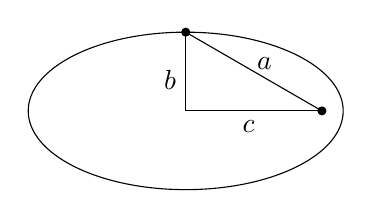
\begin{tikzpicture}[scale=1]
						\pgfmathsetmacro{\o}{0}
						\draw (0,\o) ellipse (2 and 1);
						\draw (0,\o) -- (1.73,\o);
						\draw (0,0) -- (0,1);
						\draw [fill=black] (0,1) circle (0.05);
						\draw [fill=black] (1.73,0) circle (0.05);
						\draw (0,1) -- (1.73,0);
						\node at (-0.2,0.4) [anchor=center] {\( b \)};
						\node at (0.8,-0.2) [anchor=center] {\( c \)};
						\node at (1,0.6) [anchor=center] {\( a \)};
					\end{tikzpicture}
				\end{center}
				\caption{Distance from center to focus for an ellipse.}
				\label{figH}
			\end{figure}
			From this, using the Pythagorean theorem, the following equation is derived:
			\begin{equation}
				c=\sqrt{a^2-b^2}
				\label{eqc}
			\end{equation}
			Applying this offset to the parametric ellipse, the following is derived:
			\begin{equation}
				\left(x,y\right)=\left(a\cos{\left(E\right)}-c,b\sin{\left(E\right)}\right)
				\label{eqd}
			\end{equation}
			Equation \eqref{eqd} shifts the ellipse to the left, in the negative-\( x \) direction, so that the periapsis of the orbit is at \( E=\qty{0}{\radian} \). Finally, since TLEs do not contain an expression for the length of the semi-minor axis, \( b \) must be derived from \( a \) and \( e \) as follows:
			\begin{equation}
				e^2=1-\frac{b^2}{a^2}
			\end{equation}
			\begin{equation}
				\Rightarrow e^2 a^2=a^2-b^2
			\end{equation}
			\begin{equation}
				\Rightarrow b=\sqrt{a^2-e^2 a^2}
			\end{equation}
			Then, using \eqref{eqc}, the following is derived:
			\begin{equation}
				c=ea
			\end{equation}
			\begin{equation}
				\therefore \left(x,y\right)=\left(a\cos{\left(E\right)}-ea,\sqrt{a^2-e^2 a^2}\sin{\left(E\right)}\right)
			\end{equation}
			From this, various 3D rotations are performed in on the ellipse around the origin in order to achieve the final orbit ellipse.

			Out of the classical orbital elements, \( i \), \( \Omega \), and \( \omega \) are the rotational elements: \( i \) rotates the orbit around the line of nodes; \( \Omega \) rotates the orbit around the barycenter in the celestial equatorial plane; and \( \omega \) rotates the orbit around the barycenter in the orbital plane. Thus, the simplest order of rotations would be to first rotate the ellipse in the orbital plane, so that it is a simple 2-dimensional rotation, then rotate the entire orbital plane around the line of nodes, which would be colinear with the \( \vhat{I} \) axis at this point, and then finally rotate the line of nodes and the orbital plane around the origin, which would essentially be another 2-dimensional rotation, keeping all of the \( \vhat{K} \) components static.
			\begin{figure}[hbtp]
				\begin{center}
					\tdplotsetmaincoords{0}{0}
					\begin{tikzpicture}[tdplot_main_coords, scale=2]
						\draw [->] (0,0) -- (1,0) node [anchor=west] {\( x \)};
						\draw [->] (0,0) -- (0,1) node [anchor=south] {\( y \)};
						\tdplotsetrotatedcoords{30}{0}{0}
						\draw [tdplot_rotated_coords, ->] (0,0) -- (1,0) node [anchor=south west] {\( P \)};
						\tdplotsetrotatedcoords{60}{0}{0}
						\draw [tdplot_rotated_coords, ->] (0,0) -- (1,0) node [anchor=south west] {\( P^\prime \)};
						\tdplotdrawarc[color=red, ->]{(0,0,0)}{0.75}{0}{30}{anchor=west}{\( \theta \)}
						\tdplotdrawarc[color=Purple2, ->]{(0,0,0)}{0.65}{30}{60}{anchor=south west}{\( \phi \)}
					\end{tikzpicture}
				\end{center}
				\caption{2D rotation.}
				\label{figI}
			\end{figure}
			From Fig.~\ref{figI} and the following equations, it is demonstrated that, given an initial point of a graph \( P \), and a desired rotation \( \phi \), a desired final point \( P^\prime \) can be achieved:
			\begin{equation}
				P^\prime=
				\begin{cases}
					x^\prime=r\cos{\left(\theta\right)}\cos{\left(\phi\right)}-r\sin{\left(\theta\right)}\sin{\left(\phi\right)}\\
					y^\prime=r\cos{\left(\theta\right)}\sin{\left(\phi\right)}+r\sin{\left(\theta\right)}\cos{\left(\phi\right)}
				\end{cases}
			\end{equation}
			\begin{equation}
				P=
				\begin{cases}
					x=r\cos{\left(\theta\right)}\\
					y=r\sin{\left(\theta\right)}
				\end{cases}
			\end{equation}
			\begin{equation}
				\therefore P^\prime=
				\begin{cases}
					x^\prime=x\cos{\left(\phi\right)}-y\sin{\left(\phi\right)}\\
					y^\prime=x\sin{\left(\phi\right)}+y\cos{\left(\phi\right)}
				\end{cases}
				\label{eqaaa}
			\end{equation}
			Applying \eqref{eqaaa} to the base orbital ellipse as a rotation of \( \omega \), a rotation matrix \( \bm{\left[R_{\omega}\right]} \) can be derived:
			\begin{equation}
				\bm{\left[R_{\omega}\right]}=
				\begin{bmatrix}
					\cos{\left(\omega\right)} & -\sin{\left(\omega\right)}\\
					\sin{\left(\omega\right)} & \cos{\left(\omega\right)}
				\end{bmatrix}
				\label{eq1}
			\end{equation}
			Equation \eqref{eq1} rotates the orbital ellipse, and by extension the periapsis, around the barycenter, so that the periapsis is \( \omega \) away from \( \ascnode \) in the direction of the orbit, thus achieving the desired effect of the orbital element \( \omega \), as demonstrated in Fig.~\ref{figJ} and Fig.~\ref{figK}.

			\begin{figure}[hbtp]
				\begin{center}
					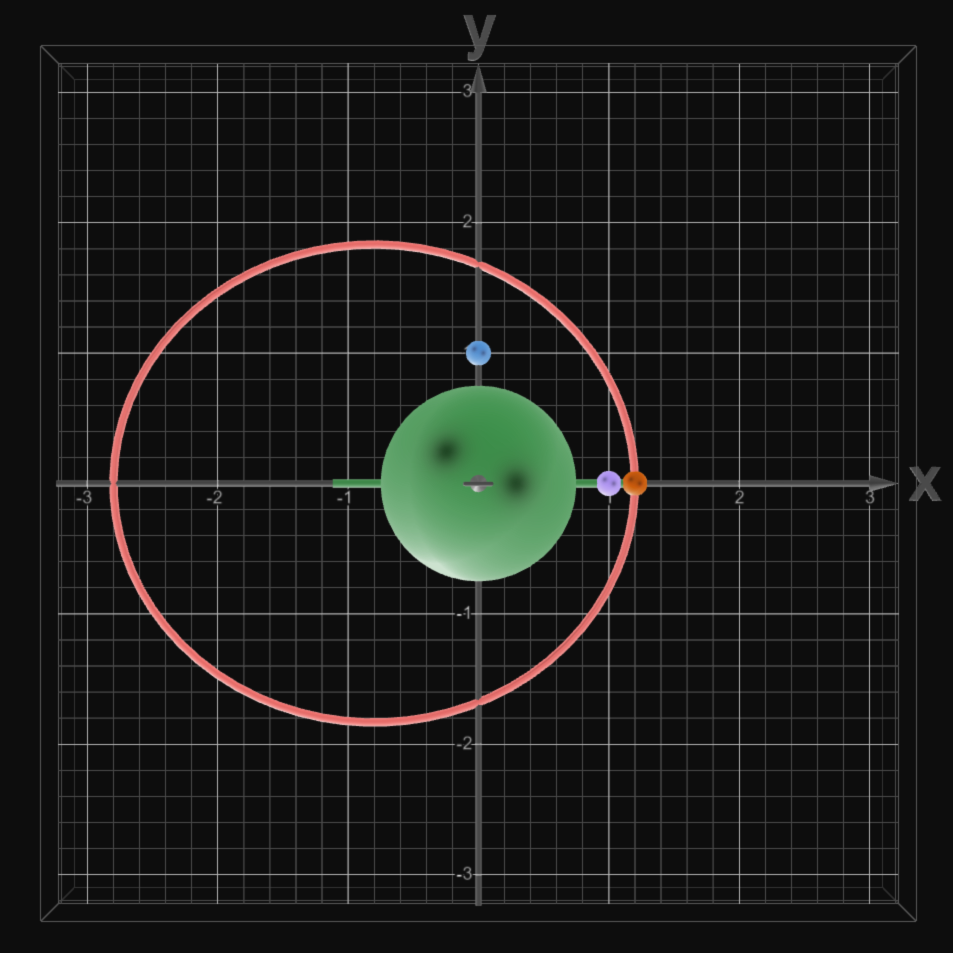
\includegraphics[width=0.8\columnwidth]{1.png}
				\end{center}
				\caption{Orbital ellipse before \( \bm{\left[R_{\omega}\right]} \).}
				\label{figJ}
			\end{figure}

			\begin{figure}[hbtp]
				\begin{center}
					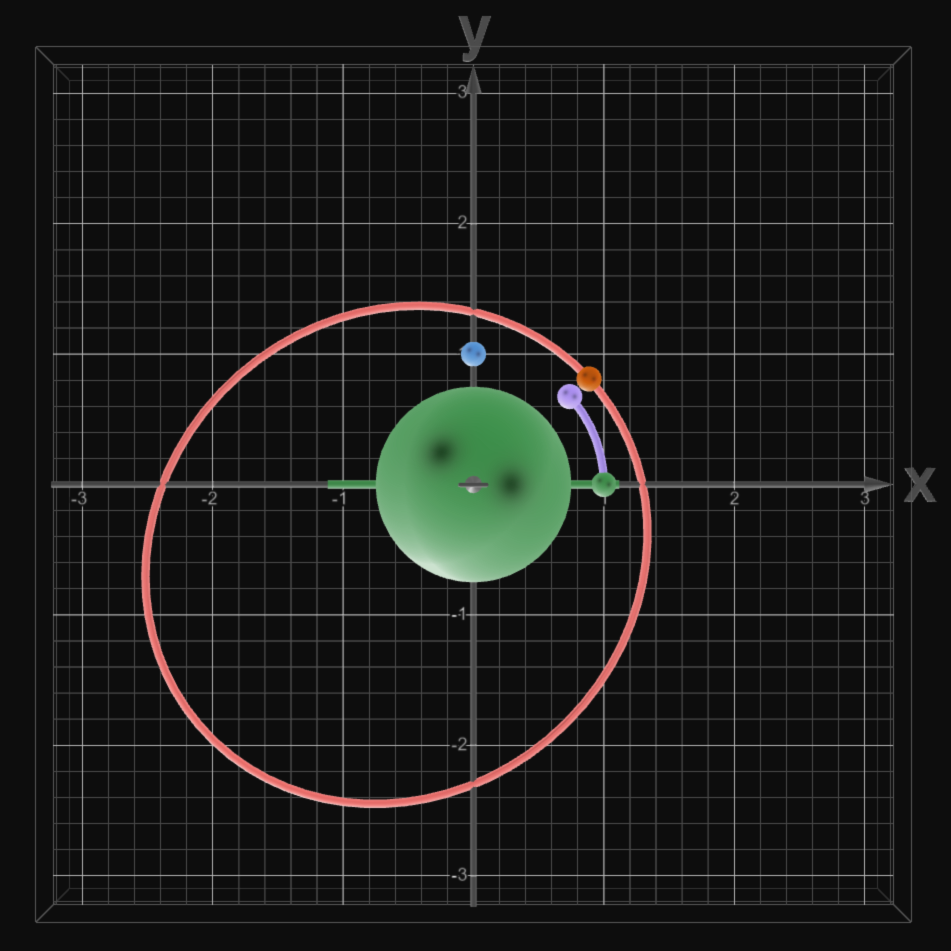
\includegraphics[width=0.8\columnwidth]{2.png}
				\end{center}
				\caption{Orbital ellipse after \( \bm{\left[R_{\omega}\right]} \).}
				\label{figK}
			\end{figure}

			Next, the entire orbital plane must be rotated around the line of nodes. In its current state, the line of nodes is colinear with the \( x \)-axis, meaning rotating the graph's \( yz \)-plane around the origin would achieve the desired effect. Thus, using the output 2-dimensional vector of the last matrix as the input for the next matrix, a rotation matrix \( \bm{\left[R_i\right]} \) can be derived. Given that the \( z \)-component of the input vector is zero, since the base orbital plane is only in the \( xy \)-plane, the third column of \( \bm{\left[R_i\right]} \) can be omitted:
			\begin{equation}
				\bm{\left[R_i\right]}=
				\begin{bmatrix}
					1 & 0\\
					0 & \cos{\left(i\right)}\\
					0 & \sin{\left(i\right)}
				\end{bmatrix}
				\label{eq2}
			\end{equation}
			Equation \eqref{eq2} rotates the orbital plane around the line of nodes, so that the orbital plane is \( i \) away from the celestial equatorial plane, achieving the desired result, as demonstrated in Fig.~\ref{figL} and Fig.~\ref{figM}.

			\begin{figure}[hbtp]
				\begin{center}
					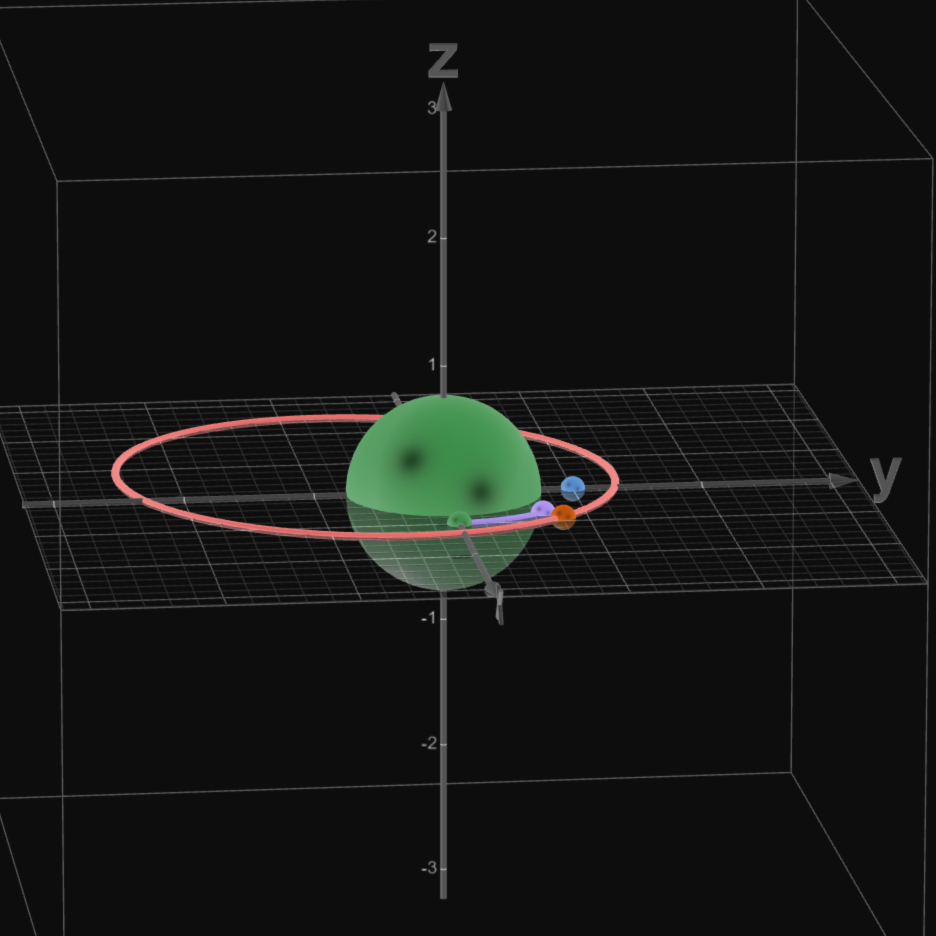
\includegraphics[width=0.8\columnwidth]{3.png}
				\end{center}
				\caption{Orbital ellipse before \( \bm{\left[R_i\right]} \).}
				\label{figL}
			\end{figure}

			\begin{figure}[hbtp]
				\begin{center}
					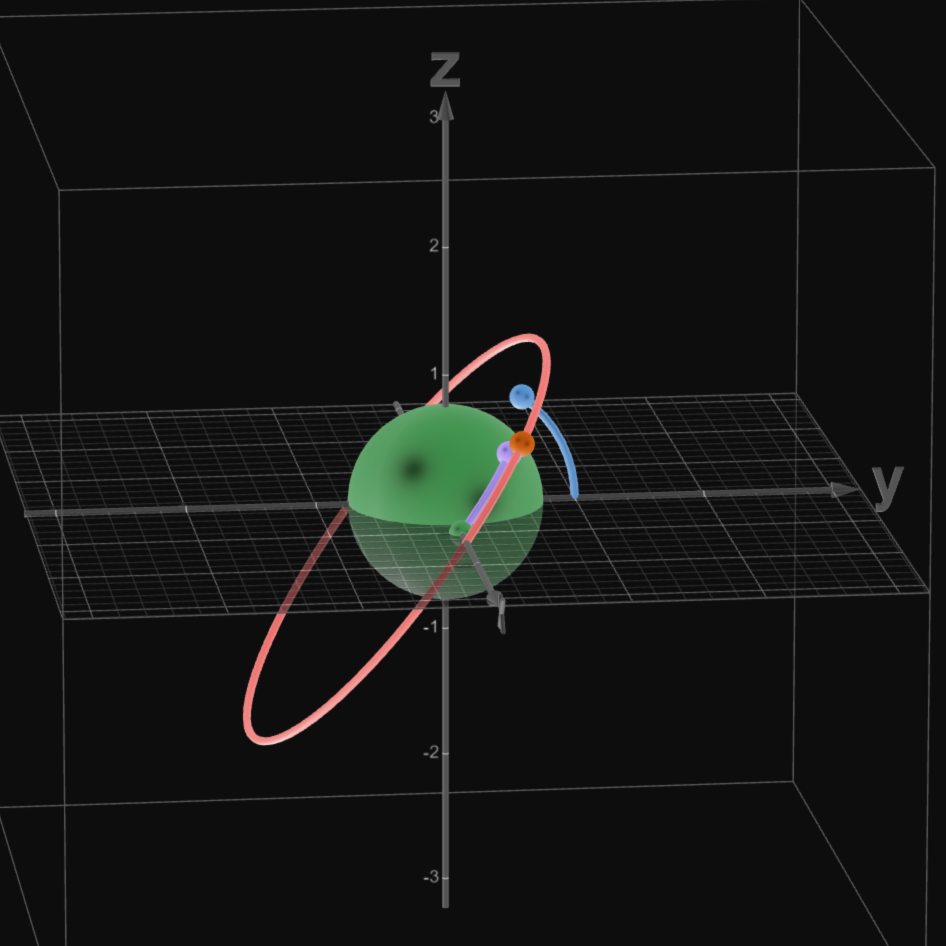
\includegraphics[width=0.8\columnwidth]{4.png}
				\end{center}
				\caption{Orbital ellipse after \( \bm{\left[R_i\right]} \).}
				\label{figM}
			\end{figure}

			Finally, the result of \eqref{eq2} must be rotated around the \( z \)-axis. Since this is simply another rotation of the \( xy \)-plane without affecting the \( z \)-component of any coordinate, a rotation matrix similar to that of \eqref{eq1}, \( \bm{\left[R_{\Omega}\right]} \), can be employed:
			\begin{equation}
				\bm{\left[R_{\Omega}\right]}=
				\begin{bmatrix}
					\cos{\left(\Omega\right)} & -\sin{\left(\Omega\right)} & 0\\
					\sin{\left(\Omega\right)} & \cos{\left(\Omega\right)} & 0\\
					0 & 0 & 1
				\end{bmatrix}
				\label{eq3}
			\end{equation}
			Equation \eqref{eq3} rotates the entire orbit around the celestial pole, so that the line of nodes is \( \Omega \) away from \( \aries \), achieving the desired result, as demonstrated in Fig.~\ref{figN} and Fig.~\ref{figO}.

			\begin{figure}[hbtp]
				\begin{center}
					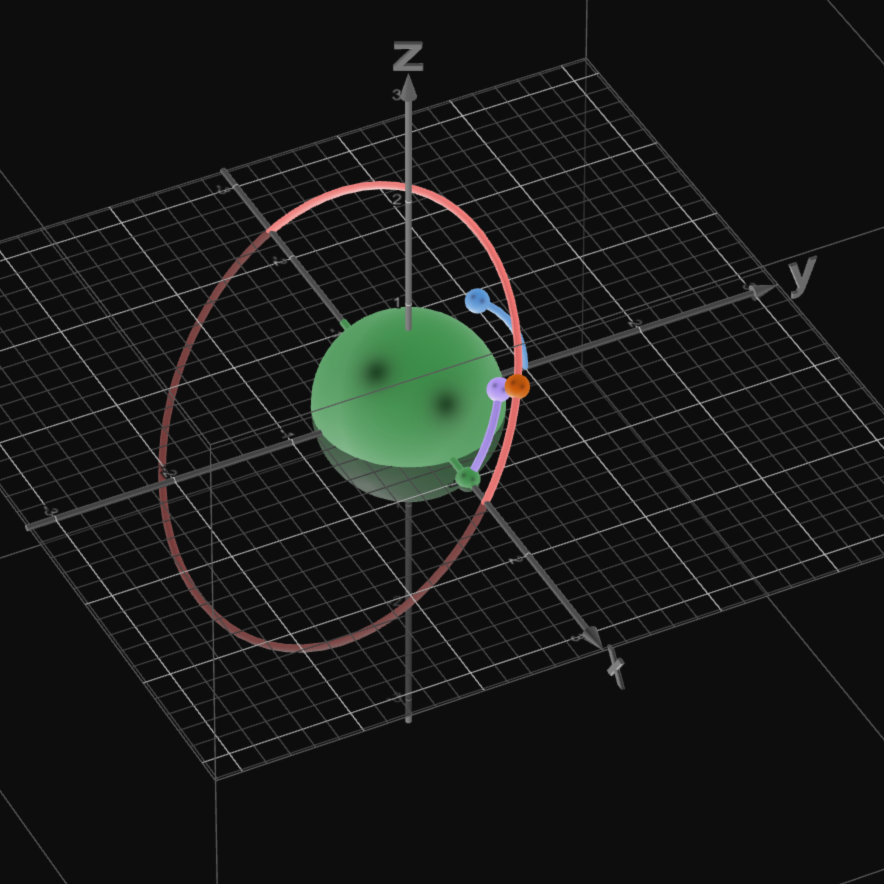
\includegraphics[width=0.8\columnwidth]{5.png}
				\end{center}
				\caption{Orbital ellipse before \( \bm{\left[R_{\Omega}\right]} \).}
				\label{figN}
			\end{figure}

			\begin{figure}[hbtp]
				\begin{center}
					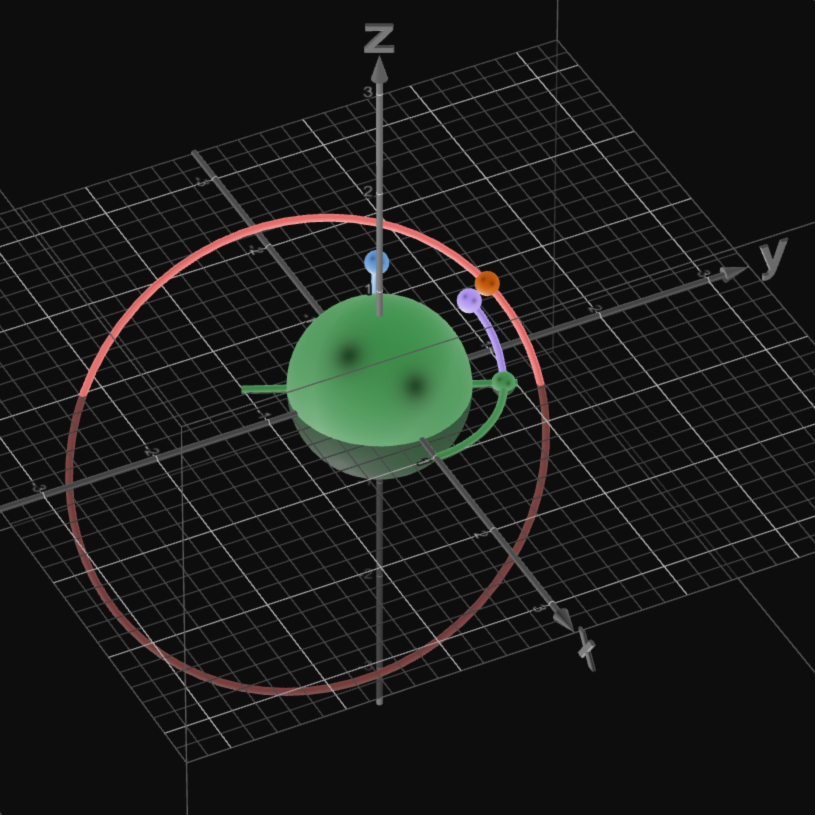
\includegraphics[width=0.8\columnwidth]{6.png}
				\end{center}
				\caption{Orbital ellipse after \( \bm{\left[R_{\Omega}\right]} \).}
				\label{figO}
			\end{figure}

			Putting all of these rotation matrices together, the following equation describes the entire translation from a simple ellipse drawn from \( a \) and \( e \) to a 3-dimensional orbit of a satellite.
			\begin{equation}
				\left\langle
					\begin{matrix}
						I\\
						J\\
						K
					\end{matrix}
				\right\rangle
				=\bm{\left[R_{\Omega}\right]}\bm{\left[R_i\right]}\bm{\left[R_{\omega}\right]}
				\left\langle
					\begin{matrix}
						a\cos{\left(E\right)}-c\\
						b\sin{\left(E\right)}
					\end{matrix}
				\right\rangle
				\label{eq4}
			\end{equation}

		\subsection{Implementation in Unity}
			The resulting matrices and equations from Desmos are replicated using the \texttt{Mathf} class in the main satellite script, \texttt{orbit.cs}, within Unity. The \texttt{cameraMovement.cs} script is attached to the main camera object; the \texttt{readTLE.cs} script is attached to the textbox object; and the \texttt{orbit.cs} script is attached to the satellite object. This then concludes the main effort of the project. Aside from the main deliverable, additional features were also added, such as a rotating Earth, a start button, an exit button, and a textual display for all six classical orbital elements.

			The rotation of the Earth is set based on the framerate of the program, so that it also matches the rotation of the satellite. In testing, using the International Space Station's TLE, through one full rotation of the Earth, the satellite object completed approximately \( 15.5 \) orbits, which is consistent with the actual International Space Station, confirming the periodic accuracy of the program.

	\section{Conclusion}

		\subsection{Project Deliverables}
			The final deliverable for the project is a Windows software tool, built in Unity, that takes in a TLE as an input and creates a 3D model of the orbit of the satellite that the TLE corresponds to, in an interactive 3D environment. A brief guide on how to use the tool is also included as a deliverable at the end of this document.

		\subsection{Challenges and Difficulties}
			Many challenges and difficulties were faced throughout the development of this project. Chiefly among those were learning Unity for the first time and understanding all of the relationships and quirks in the Unity object management system, deconstructing all six of the classical orbital elements into something comprehensible, and developing a coherent set of rotation matrices to represent those orbital elements.

			Additionally, the major time constraint of needing to finish such a large project in less than half a semester, while also spending time on other courses, proved to be incredibly challenging.

		\subsection{Thoughts on Project and Future Development}
			For additional development in the future, I would like to add in all of the visual elements that I did not have time to add into this initial release of the project, such as all of the visualizations of the orbital elements as seen in the Desmos figures, as well as a transparent cone to demonstrate where geographically a satellite would be able to communicate with.

	\section*{Usage Information and Notes}
		The program is started by running the \texttt{Satellite Visualizer.exe}.

		A TLE can be entered or pasted into the textbox labeled \texttt{ENTER TLE:}.

		The camera is moved via \texttt{WASD, Space, L Shift} and the mouse.

		Clicking the green button labeled \texttt{START} after having input a valid TLE will begin all rotations and orbits.

		Clicking the red button labeled \texttt{CLOSE PROGRAM} will close out of the program.

		The source code for my final project can be found in the GitHub repository for this project: \url{https://github.com/Veloraxzia-Tenebris/Satellite-Visualizer.git}. The playable release can be found here: \url{https://github.com/Veloraxzia-Tenebris/Satellite-Visualizer/releases/tag/v1.0.0}
\end{document}